\documentclass[a4paper]{article}
\usepackage[utf8]{inputenc}
\usepackage[spanish, es-tabla]{babel}

\usepackage{amsmath}
\usepackage{amsfonts}
\usepackage{amssymb}

\usepackage{float}
\usepackage{graphicx}
\graphicspath{ {./Imagenes/} }

\usepackage{multirow}
\setlength{\doublerulesep}{\arrayrulewidth}

\usepackage{array}
\newcolumntype{C}[1]{>{\centering\let\newline\\\arraybackslash\hspace{0pt}}m{#1}}

\usepackage[american]{circuitikz}

\usepackage{fancyhdr}

\usepackage{units} 

\pagestyle{fancy}
\fancyhf{}
\lhead{22.42 Laboratorio de Electrónica}
%\rhead{Bertachini, Lambertucci, Londero, Mechoulam}
\rfoot{Página \thepage}



\begin{document}

%%%%%%%%%%%%%%%%%%%%%%%%%%%%%%%%%%%%%%%%%%%%%%%%%%%%%%%%%%%%%%%%%%%%%%%%% 
%								CARATULA								%
%%%%%%%%%%%%%%%%%%%%%%%%%%%%%%%%%%%%%%%%%%%%%%%%%%%%%%%%%%%%%%%%%%%%%%%%% 

\begin{titlepage}

\newcommand{\HRule}{\rule{\linewidth}{0.5mm}}
\center
\mbox{\textsc{\large \bfseries {INSTITUTO TECNOLÓGICO DE BUENOS AIRES}}}\\[1cm]
\textsc{\Large 22.42 Laboratorio de Electrónica}\\[0.5cm]


\HRule \\[0.6cm]
{ \Huge \bfseries Trabajo Práctico N$^{\circ}$4}\\[0.4cm] 
\HRule \\[1.5cm]


{\large

\emph{Grupo 3}\\
\vspace{3px}

\begin{tabular}{lr} 	
\textsc{Bertachini}, Germán  & 58750 \\ 	
\textsc{Lambertucci}, Guido Enrique  & 58009 \\
\textsc{Londero Bonaparte}, Tomás Guillermo  & 58150 \\
\textsc{Mechoulam}, Alan  &  58438\\
\textsc{Scapolla}, Franco & 58465
\end{tabular}

\vspace{20px}

\emph{Profesores}\\
\vspace{3px}
\textsc{Cossutta}, Pablo Martín\\
\textsc{Weill}, María\\
\textsc{Salvati}, Matías\\	
\vspace{100px}

\begin{tabular}{ll}

Presentado: & 15/10/19\\

\end{tabular}

}

\vfill

\end{titlepage}



%%%%%%%%%%%%%%%%%%%%%%%%%%%%%%%%%%%%%%%%%%%%%%%%%%%%%%%%%%%%%%%%%%%%%%%%% 
%								INFORME									%
%%%%%%%%%%%%%%%%%%%%%%%%%%%%%%%%%%%%%%%%%%%%%%%%%%%%%%%%%%%%%%%%%%%%%%%%%

\section*{Introducción}

En el siguiente informe se realizan diversas mediciones con el osciloscopio, con el objetivo de mejorar el manejo y comprensión de dicho instrumento.

\section*{Desarrollo de la experiencia}

\subsection*{Filtro pasabajos de primer orden}

Se realiza en un protoboard el circuito mostrado en la figura (\ref{graf:pasabajos}). Para esto se utilizó una resistencia $ R = 3,9 \ k\Omega $ y un capacitor $ C = 2,2 \ nF $. Ademas, se utilizó el analizador de impedancia con ambos componentes para medir sus valores reales obteniendose así los siguientes valores medidos: $ R_{m} = 3,87 \ k\Omega $ y $ C_{m} = 2,24 \ nF $.

\begin{figure}[H]
	\centering
	\includegraphics[width=0.9\textwidth]{Filtro-pasabajos.PNG}
	\caption{Filtro pasabajos.} 
	\label{graf:pasabajos}
\end{figure}

Con la fuente, se aplicó una tensión senoidal de una amplitud de $9,78 \ V$ para determinar la frecuencia de resonancia real de dicho circuito, obteniéndose así una frecuencia de $18,5 \ k\ Hz$. Luego, midiéndose la tensión del capacitor, se busca calcular el valor de capacitancia y de esta forma calcular el error existente entre el valor de calculado de esta forma y el obtenido por el analizador de impedancia. Utilizando el valor teórico de la resistencia se obtiene $2,21  \ nF  $, mientras que con el valor medido $2,23  \ nF  $. Se retira el capacitor y se repiten las mediciones realizadas con el objetivo de calcular la capacidad de las puntas del osciloscopio. De esta forma se obtiene un error de $ ???  $ con el valor teórico de la resistencia, y un error de $  ???  $ con el medido.
A continuación, se mide la diferencia de fase entre la corriente y la tensión en el capacitor, y se verifica la suma vectorial de las tensiones, es decir $ \overrightarrow{V} = \overrightarrow{V_R} \ + \ \overrightarrow{V_C} $.

%\begin{figure}[H]
%	\centering
%	\includegraphics[width=0.9\textwidth]{}
%	\caption{Suma vectorial de las tensiones del circuito.} 
%	\label{graf:sumavectorial}
%\end{figure}

Posteriormente se calcula analíticamente la transferencia del circuito, llegándose a la expresión

\begin{equation}
	H \left(S \right) = \frac{V_C}{V} = \frac{1}{SCR + 1} = \frac{1}{S \cdot 8.58 \cdot 10^{-6} + 1}
	\label{equ:transfpasabajos}
\end{equation}

Ademas, partiendo de una frecuencia de $ 10 \ Hz $ hasta llegar a $ 1 \ MHz $, se toman varios valores tanto de la tensión del capacitor como de la fuente. De esta forma, se grafica punto a punto la transferencia y se la compara con la teórica hallada en (\ref{equ:transfpasabajos}).

%\begin{figure}[H]
%	\centering
%	\includegraphics[width=0.9\textwidth]{}
%	\caption{Transferencia teórica y medida del circuito \ref{graf:pasabajos}.} 
%	\label{graf:transfpasabajos}
%\end{figure}

Luego, se mide la tensión de la resistencia ...

\subsection*{Filtro pasaaltos de primer orden}

Con los mismos elementos utilizados para armar el circuito (\ref{graf:pasabajos}), se elabora el circuito pasaaltos de la figura (\ref{graf:pasaaltos}). Su transferencia se calcula analíticamente obteniéndose:

\begin{equation}
	H \left(S \right) = \frac{V_C}{V} = \frac{SCR}{SCR + 1} = \frac{S \cdot 8.58 \cdot 10^{-6}}{S \cdot 8.58 \cdot 10^{-6} + 1}
	\label{equ:transfpasaaltos}
\end{equation}

\begin{figure}[H]
	\centering
	\includegraphics[width=0.9\textwidth]{Filtro-pasaaltos.PNG}
	\caption{Filtro pasabaltos.} 
	\label{graf:pasaaltos}
\end{figure}

Al igual que con el filtro pasabajos, se procede a medir varios puntos de la tensión de la resistencia y de la fuente, variando la frecuencia. Así se grafica la transferencia medida y se la compara con la teórica hallada en (\ref{equ:transfpasaaltos}).

A continuación, se reemplaza la tensión sinusoidal por una triangular, variando la frecuencia. ...

\textbf{Mostrar 3 gráficos representativos y sacar conclusiones. En el caso mas apropiado medir la respuesta transitoria y en caso de ser viable, demostrar analíticamente lo obtenido}

\subsection*{Sincronización de instrumentos}
En este punto se utiliza el barrido automático del generador de funciones, para visualizar en el osciloscopio la respuesta en frecuencia del circuito de la la figura (\ref{graf:pasabajos}). Por un lado, se realizó dicha medición utilizando el modo XY, es decir, se utilizaron dos generadores. Mientras que con uno se genera la rampa correspondiente al canal X, con el otro se genera el barrido. ...
Por otro lado, también se utilizó el modo normal, disparado acordemente, es decir, utilizando un solo generador de funciones.

\subsection*{Respuesta en frecuencia del osciloscopio}
Finalmente, se midió la respuesta en frecuencia de un cierto osciloscopio (MARCA Y MODELO DEL OSCILOSCOPIO), activando los filtros AC y BW. Se esperaba, según la teoría, que la respuesta sea similar a la de un filtro pasa-banda, atenuando las frecuencias muy bajas y muy altas. Esto es, realizando a priori la suposición de que el generador de funciones nos proporcionará una amplitud de señal constante a todas las frecuencias.

Para realizar la medición, se conectó el osciloscopio con las puntas en x10 previamente calibradas, se activaron los filtros y se conectaron las puntas del osciloscopio a la salida de un generador de funciones con una señal sinusoidal de amplitud pico a pico de 20 voltios. Se comenzó a medir desde la frecuencia más pequeña del generador, de $1 / Hz$, hasta la mayor frecuencia que admite el generador, de $15 / MHz$.

\begin{figure}[H]
	\centering
	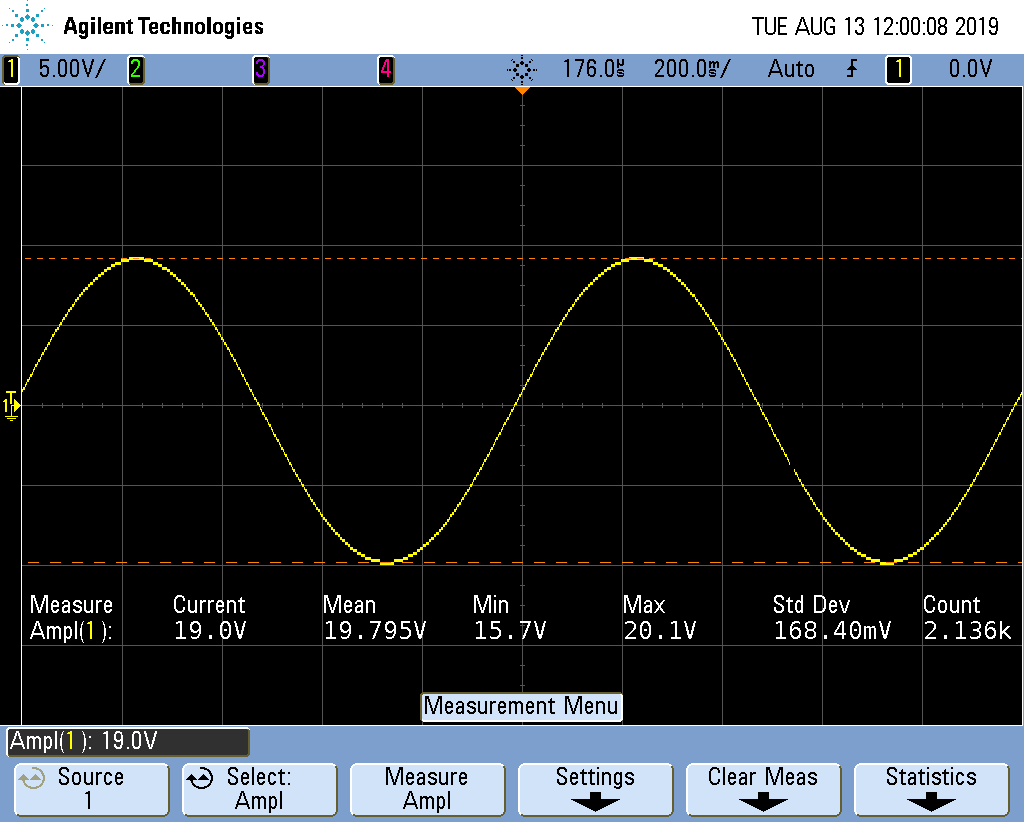
\includegraphics[width=0.8\textwidth,trim={0.7cm 5cm  0.5 8cm},clip]{osci1hz.png}
	\caption{Medición de la respuesta en frecuencia del osciloscopio a una frecuencia de $1 \ Hz$ con los filtros BW y AC. (500ms/div)} 
	\label{graf:osci_freq_baja}
\end{figure}

\begin{figure}[H]
	\centering
	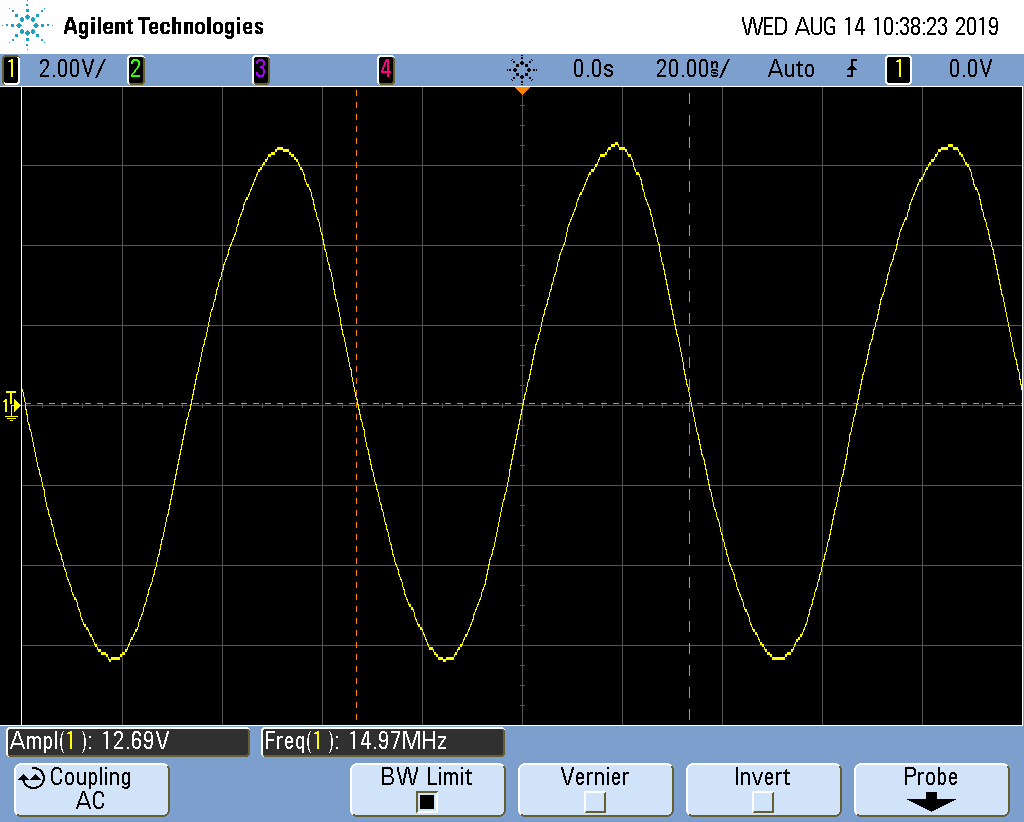
\includegraphics[width=0.8\textwidth,trim={0.7cm 5cm  0.5 8cm},clip]{osci15mhz.png}
	\caption{Medición de la respuesta en frecuencia del osciloscopio a una frecuencia de $15 \ MHz$ con los filtros BW y AC.} 
	\label{graf:osci_freq_alta}
\end{figure}


Finalmente, se logró capturar la respuesta en frecuencia en amplitud del osciloscopio con los filtros BW y AC.

\begin{figure}[H]
	\centering
	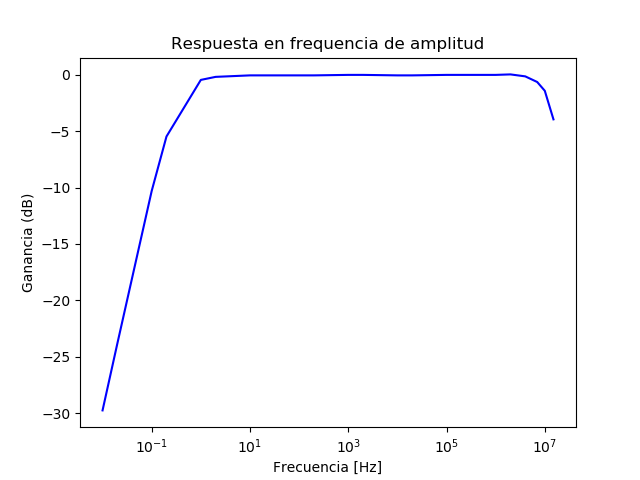
\includegraphics[width=0.8\textwidth]{resp_freq_osci.png}
	\caption{Medición de la respuesta en frecuencia del osciloscopio a una frecuencia de $1 \ Hz$ con los filtros BW y AC.} 
	\label{graf:resp_freq_osci}
\end{figure}

Se puede observar que en la práctica la respuesta en frecuencia del osciloscopio resulta ser un pasabanda, que atenua frecuencias menores a $10 \ Hz$ y mayores a $\approx 1 \ MHz$. Estos resultados verifican la suposición hecha por los conocimientos de la teoría. A continuación, se contrastan las mediciones realizadas con los datos provistos por el fabricante del osciloscopio utilizado.

\section*{Conclusión}

yo sacaria esto y pondria conclusion en cada punto por separado

\end{document}
